\documentclass[tikz, border=1mm]{standalone}

%% This is a drawing of Vámos matroid https://en.wikipedia.org/wiki/V%C3%A1mos_matroid

\begin{document}
	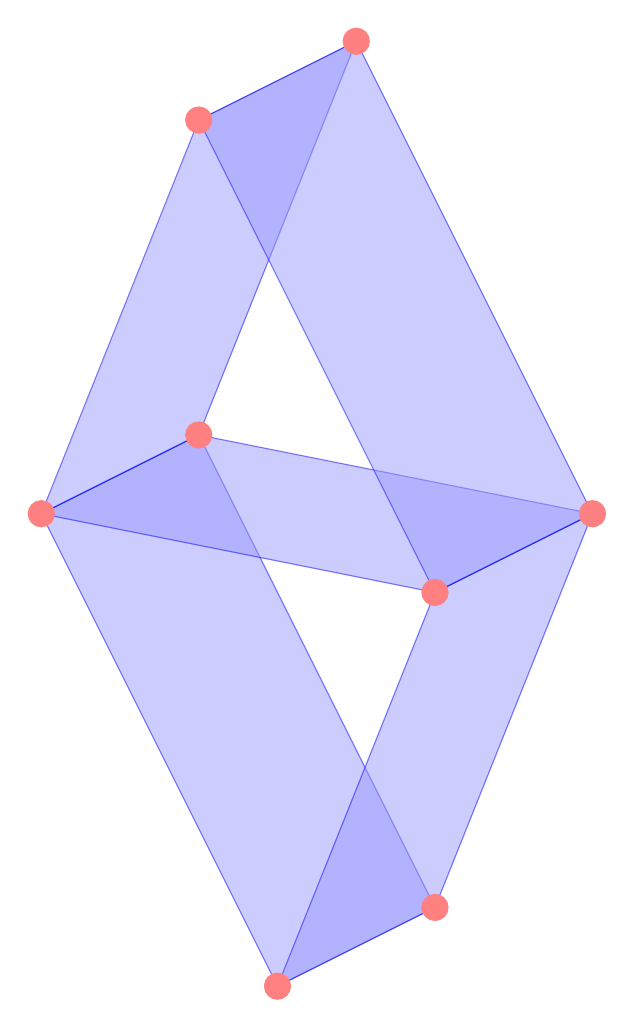
\begin{tikzpicture}[dot/.style = {draw, circle, fill, red!50}, rect/.style= {blue, fill=blue!40, opacity=0.5}]
		\coordinate (0) at (0,0);
		\coordinate (1) at (2,1);
		\coordinate (2) at (2,5);
		\coordinate (3) at (4,6);
		
		\coordinate (4) at (-3,6);
		\coordinate (5) at (-1,7);
		\coordinate (6) at (-1,11);
		\coordinate (7) at (1, 12);
		
		
		\draw[rect] (0) -- (1) -- (5) -- (4) -- cycle;
		\draw[rect] (0) -- (1) -- (3) -- (2) -- cycle;
		\draw[rect] (4) -- (5) -- (3) -- (2) -- cycle;
		\draw[rect] (4) -- (5) -- (7) -- (6) -- cycle;
		\draw[rect] (2) -- (3) -- (7) -- (6) -- cycle;
		
		\node[dot] at (0) {};
		\node[dot] at (1) {};
		\node[dot] at (2) {};
		\node[dot] at (3) {};
		
		\node[dot] at (4) {};
		\node[dot] at (5) {};
		\node[dot] at (6) {};
		\node[dot] at (7) {};
	\end{tikzpicture}
\end{document}
